% Generated from the checksum-bound current material atlas.
\clearpage
\section{Procedural material space}
\label{sec:material-space}
\subsection{Production bindings and sampling protocol}
The material atlas covers all 36 architectural/object surface roles, with the Floor role split into timber, carpet and stone, plus a dedicated rug program: 39 rows. Each row records 256 consecutive material seeds, for 9,984 recipe records. The finish selector is the production seeded selector, not a round-robin assignment. Six fixed illustration seeds (0, 1, 4, 19, 53, 101) supply 234 native PBR renders, matched normal renders and base-color, tangent-normal and roughness map previews. Seed four is included to illustrate frosted interior glass. The full consecutive cohort, rather than these illustrations, defines the reported frequencies; failed seeds are not replaced.

Each render uses the actual \texttt{IndoorMaterials} factory and \texttt{for\_part} binding, including palette tint, texture structure group, UV transform, clearcoat, anisotropy and transmission. The studio reuses a native Bevy renderer. Texture maps are baked by the production CPU reference implementation; this study does not measure GPU-baking throughput. The rig uses fixed 1,400/250 lux directional lights with shadows, the same seed-zero procedural reflection environment, indoor capture exposure and a $40^\circ$ vertical field of view. A 0.46 m diameter sphere and a $0.46\times0.49$ m beveled panel expose curved highlights and flat detail. Leaves use production blades with normalized atlas UVs. The backdrop is identical across columns and reveals glass transmission. These are material probes, not representative furnished rooms.

The separate assignment audit constructs every primary-room object in 256 consecutive mixed-layout rooms at density 0.65, without humans: 15007 objects and 53409 material parts. Rug fields use four bounded dye/pile slots; their bindings retain upholstery. Generic object finishes must have a valid slot in $[0,12)$ and resolve from their recorded finish seed; deliberately independent book-cover slots are retained. Food uses separately validated role-specific bindings. Per-object-category surface and slot counts are exported. This cohort checks application frequency; the studio does not estimate it. Architectural walls/floors, human skin/hair, and installation-specific facade privacy treatments are outside the object-assignment denominator. Human complexion/groom variation is not represented by these substrate probes.

\subsection{Correlated controls, bounded palettes}
Within a room, twelve finish slots share at most three texture structures per surface. Ceramic, Fabric, FabricAlt and Leather have three structures; Wood, WoodEdge, Leaf, LeafLight, LeafVariegated and Succulent have two. Other roles reuse one structure; rug fields have up to four dedicated dye/pile structures. Shared map handles bound synthesis/upload costs; independent room material seeds resample the underlying recipe. These are correlated palettes, not twelve independent textures. Painted Metal is dielectric; Chrome is conductive. Screen, phone, television, artwork, printed-paper and whiteboard maps come from their dedicated content programs. Container glass and liquids retain several fixed optical constants; their presence is not evidence of broad optical diversity.

The page pairs each image with its actual PBR scalars and seed, and exposes eight-bin observed parameter marginals and object-assignment histograms. Optional subprograms keep their own denominators. Recorded ranges include conditional controls and are not causal influence measurements. Raw base-color maps precede the material multiplier; roughness previews show the packed green channel before its scalar multiplier (or the scalar when no texture exists). Tangent normals are distinct from rendered view-space normals. The maps include production mip chains, while map previews show level zero. A fixed RGB image or parameter count cannot establish perceptual volume, photographic realism, or 10M-sample learning utility. No product-of-ranges diversity estimate is reported.

\subsection{Role inventory and realized object use}
\small
\begin{longtable}{lrrr}
\caption{Current material roles. Structures are the maximum shared map programs per room. Object parts and occupied finish slots are observed in the 256-room assignment cohort; zero means absent from that object-only cohort, not an unsupported material.}\\
\toprule Surface / floor type & Structures & Object parts & Slots seen \\\midrule
\endfirsthead
\toprule Surface / floor type & Structures & Object parts & Slots seen \\\midrule
\endhead
Paint & 1 & 100 & 0 \\
Accent & 1 & 0 & 0 \\
Wood & 2 & 2499 & 12 \\
WoodEdge & 2 & 2977 & 12 \\
FloorTimber & 1 & 0 & 0 \\
FloorCarpet & 1 & 0 & 0 \\
FloorStone & 1 & 0 & 0 \\
Ceiling & 1 & 0 & 0 \\
Metal & 3 & 9166 & 12 \\
Chrome & 3 & 1987 & 12 \\
Plastic & 3 & 8386 & 12 \\
Fabric & 3 & 590 & 12 \\
FabricAlt & 3 & 1672 & 12 \\
Glass & 1 & 0 & 0 \\
Ceramic & 3 & 1284 & 15 \\
Soil & 1 & 1116 & 0 \\
Leaf & 2 & 736 & 12 \\
LeafLight & 2 & 721 & 12 \\
Paper & 1 & 4212 & 13 \\
Screen & 1 & 426 & 12 \\
Ink & 1 & 5682 & 0 \\
Light & 1 & 443 & 0 \\
Concrete & 1 & 413 & 0 \\
Art & 1 & 1783 & 12 \\
Rubber & 1 & 5055 & 0 \\
LeafVariegated & 2 & 72 & 12 \\
Terracotta & 1 & 333 & 1 \\
Bark & 1 & 736 & 0 \\
GlassInterior & 1 & 57 & 0 \\
ContainerGlass & 1 & 399 & 0 \\
Liquid & 1 & 135 & 0 \\
Drink & 1 & 406 & 0 \\
PhoneScreen & 1 & 368 & 12 \\
PrintedPaper & 1 & 304 & 12 \\
Leather & 3 & 437 & 12 \\
Whiteboard & 1 & 232 & 12 \\
Television & 1 & 168 & 12 \\
Succulent & 2 & 308 & 12 \\
Rug & 4 & 206 & 4 \\
\bottomrule
\end{longtable}
\normalsize
Reserved fruit, crust and bread-scoring finishes are counted alongside generic object finishes, using a separate binding namespace. They retain role-specific pigments rather than arbitrary ceramic or paper colors.
\subsection{Control families}
\begin{description}
\item[Paint, accent and ceiling] Correlated scene pigment; roller, stipple, knockdown and trowel application; deposit scale, coverage, pinholes, gloss and local roughness.
\item[Timber and bark] Growth-ring warping, longitudinal/transverse grain, cut width, knots, stain pigmentation, finish absorption, pores and coating. Floor planks additionally vary board/joint scale.
\item[Textiles and leather] Weave/knit structure, yarn count and crimp, dye/pattern, pile and lustre; leather cell scale/stretch, grain, wrinkles, wear and coating. Carpet/rug pile and dye fields use separate room-scale programs, while upholstery resolves individual yarn crossings. Floor installations vary bond, basket strips, cut tint and roughness.
\item[Concrete, stone, soil and terracotta] Aggregate/grain distribution, deposits, veins, inclusions, polish and relief. The FloorStone row samples mineral mixtures rather than treating every tile as marble.
\item[Ceramic] Body/glaze mixture, pigment, gloss, clearcoat, firing variation, speckles, pooling, pinholes and crackle. Tint and texture structure are separately bound by the production factory.
\item[Botanical surfaces] Blade-aligned venation, chlorophyll patches, variegation, wax and restrained diffuse transmission. Succulent cuticles use a separate tileable pore/bloom program without blade venation.
\item[Metal, plastics, glass and content] Conductive versus painted bases, roughness and directional reflection; glass index, tint/attenuation, thickness and clear/frosted optics; independently seeded procedural screen/print content. Some constants are intentionally fixed by role.
\end{description}
\clearpage
\begin{figure}[p]
\centering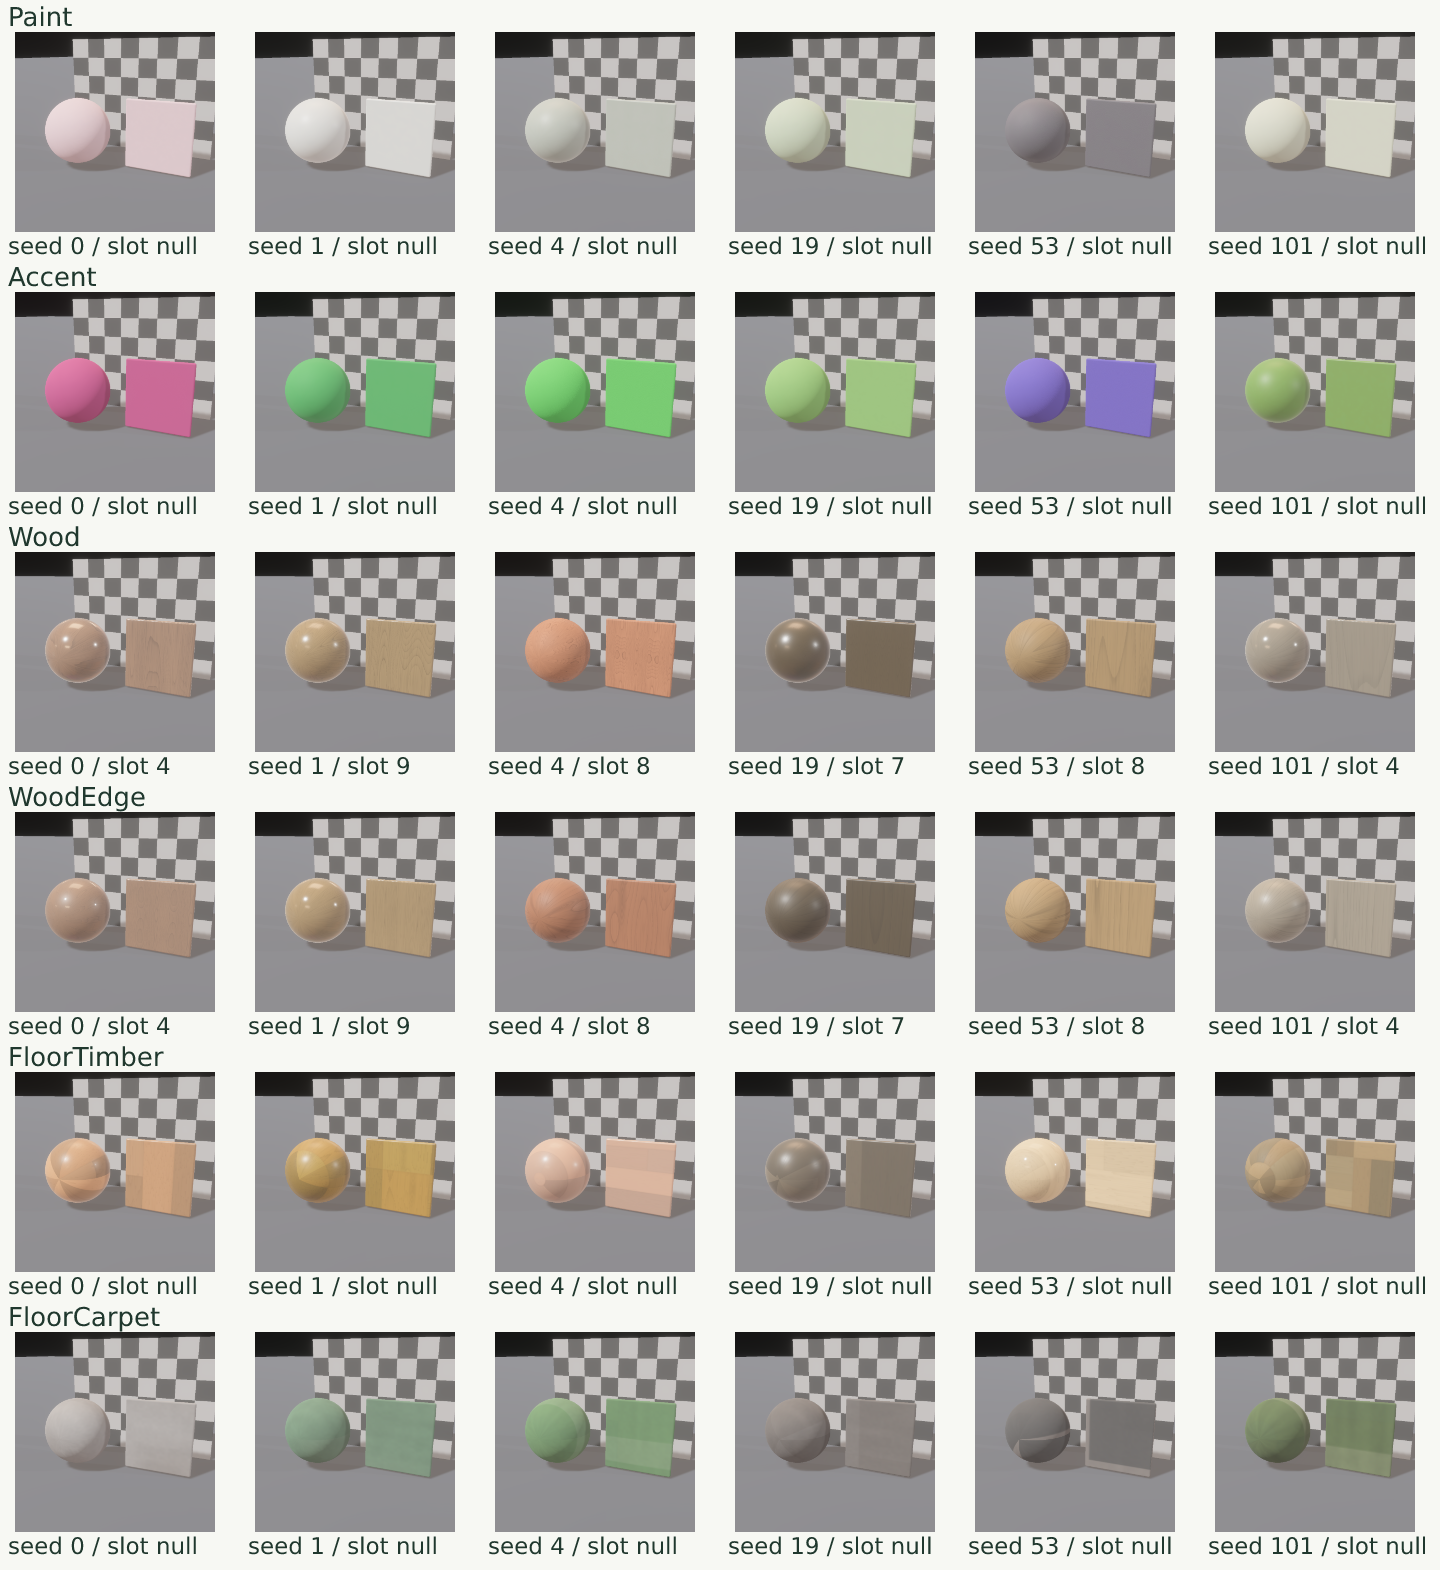
\includegraphics[width=\linewidth,height=.86\textheight,keepaspectratio]{generated/material_plate_0.png}
\caption{Native PBR material probes: Paint, Accent, Wood, WoodEdge, FloorTimber, FloorCarpet. Columns share seed, camera, lights and geometry within each row; correlated production recipes and finish slots vary. Null slots use the base role. Six fixed examples illustrate, rather than estimate, the sampled distribution. Inspect the complete 256-seed marginals, map channels and actual PBR multipliers in the project-page atlas.}
\end{figure}
\begin{figure}[p]
\centering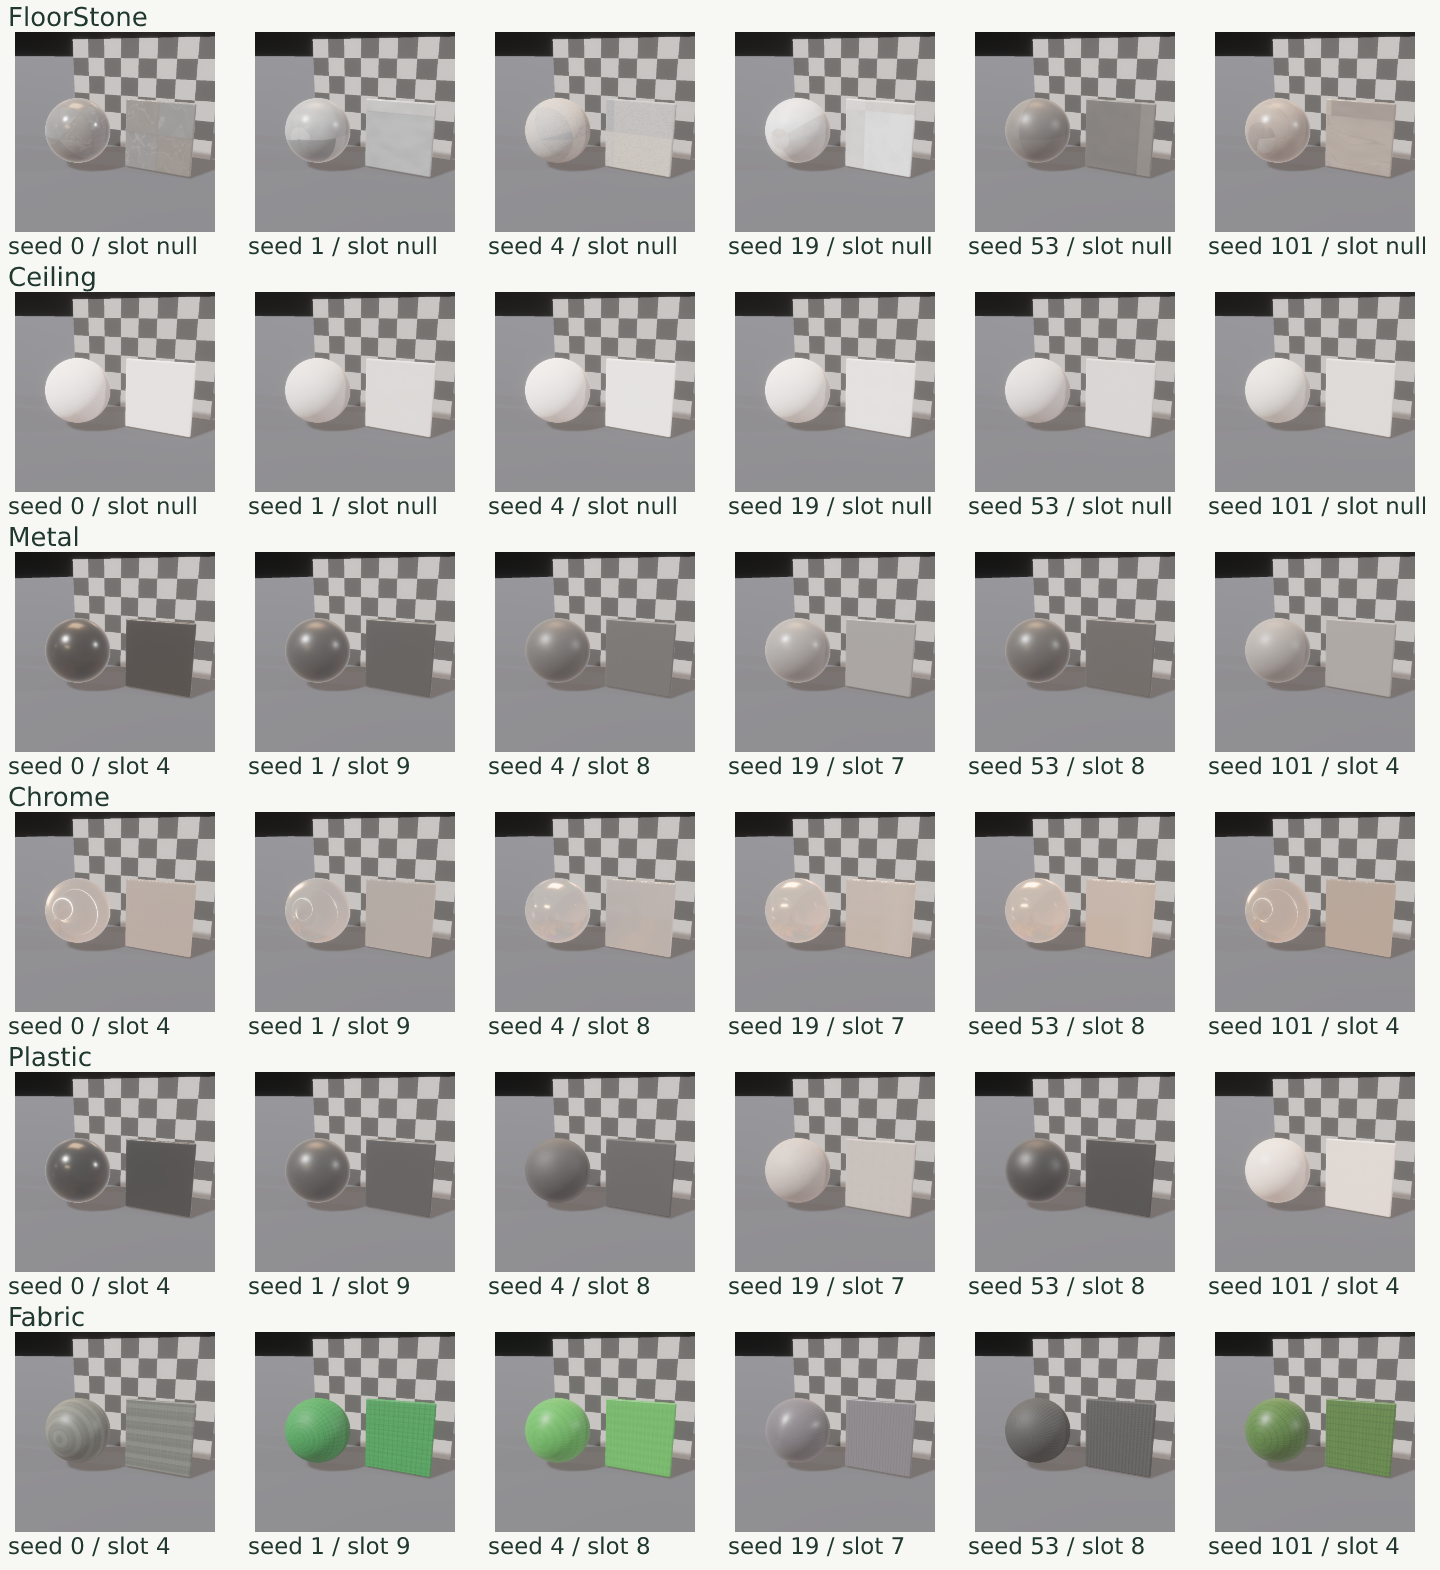
\includegraphics[width=\linewidth,height=.86\textheight,keepaspectratio]{generated/material_plate_1.png}
\caption{Native PBR material probes: FloorStone, Ceiling, Metal, Chrome, Plastic, Fabric. Columns share seed, camera, lights and geometry within each row; correlated production recipes and finish slots vary. Null slots use the base role. Six fixed examples illustrate, rather than estimate, the sampled distribution. Inspect the complete 256-seed marginals, map channels and actual PBR multipliers in the project-page atlas.}
\end{figure}
\begin{figure}[p]
\centering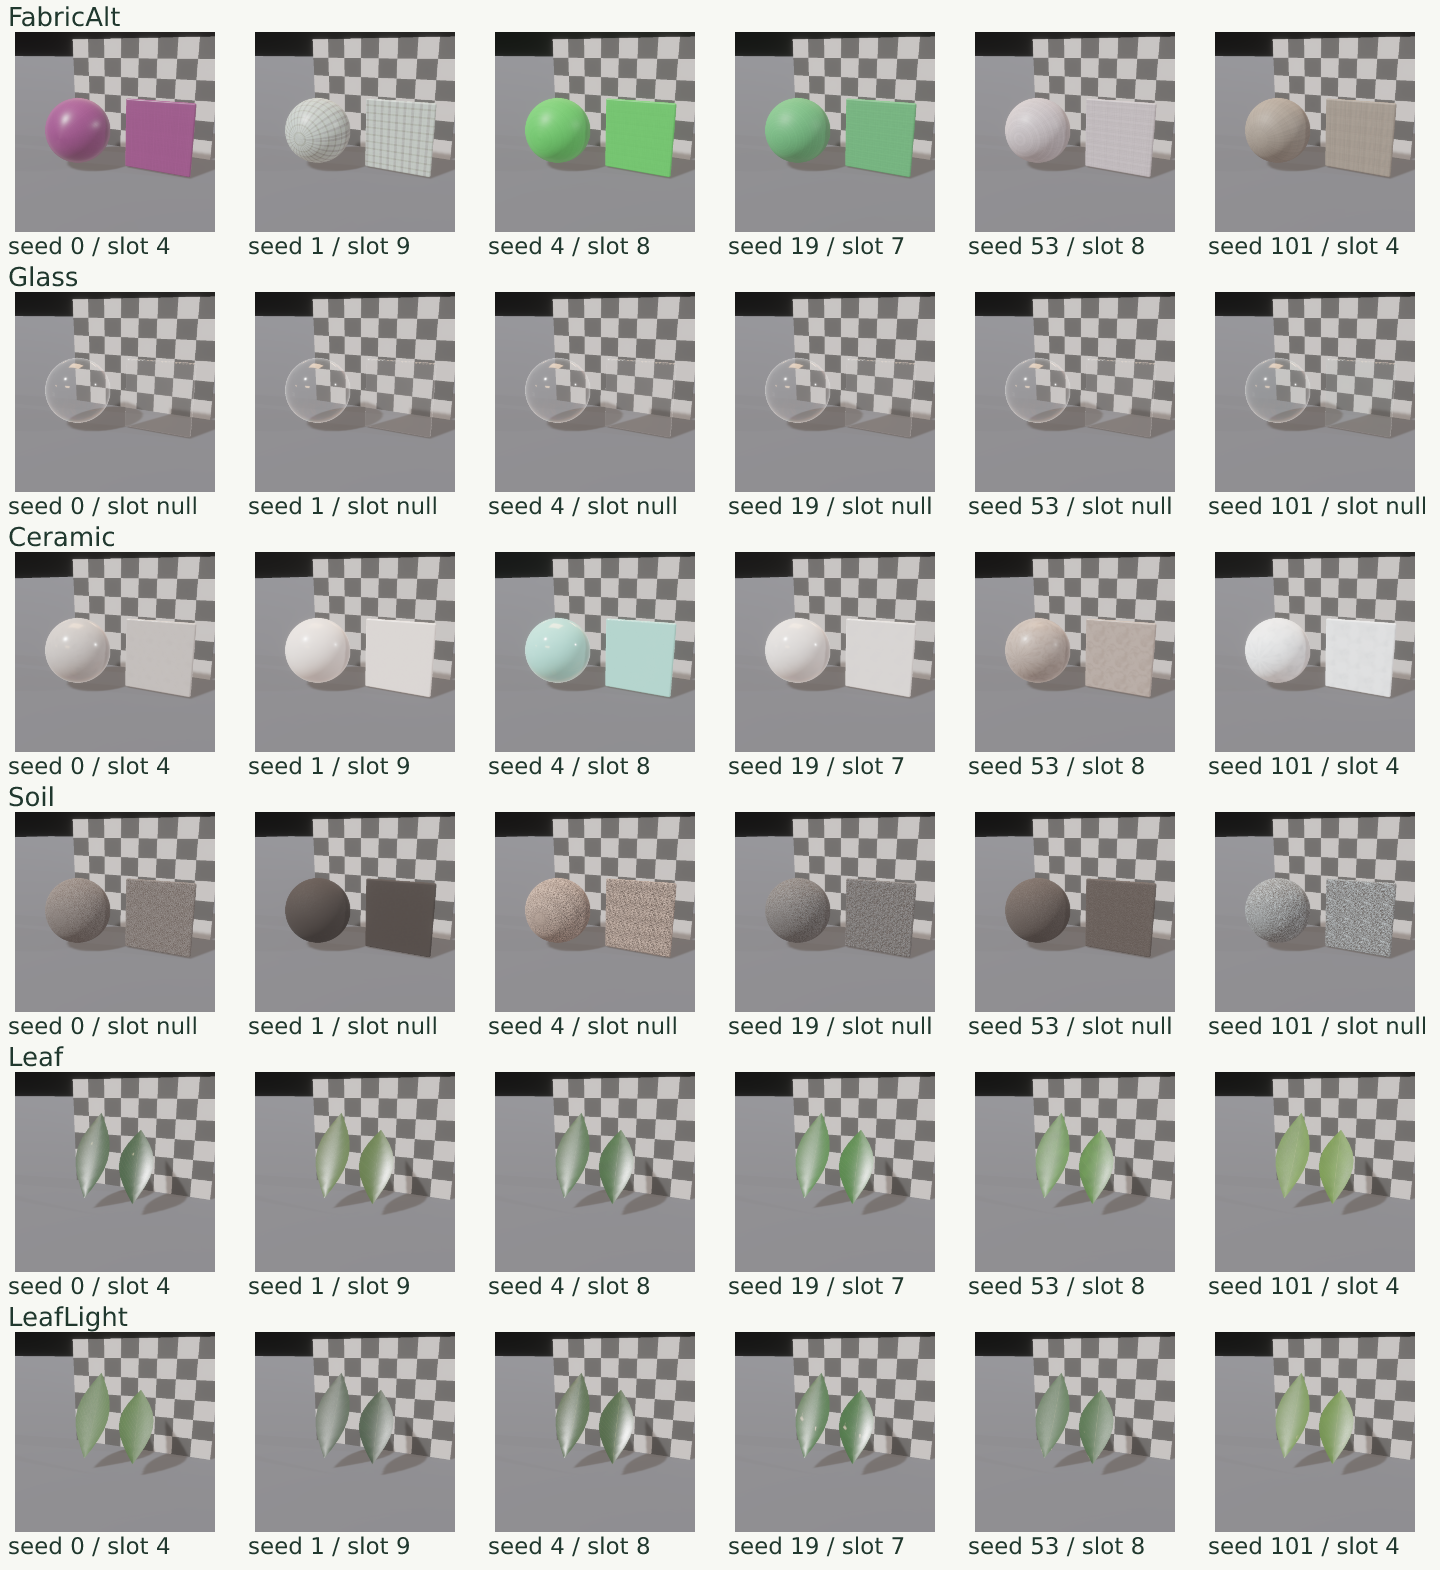
\includegraphics[width=\linewidth,height=.86\textheight,keepaspectratio]{generated/material_plate_2.png}
\caption{Native PBR material probes: FabricAlt, Glass, Ceramic, Soil, Leaf, LeafLight. Columns share seed, camera, lights and geometry within each row; correlated production recipes and finish slots vary. Null slots use the base role. Six fixed examples illustrate, rather than estimate, the sampled distribution. Inspect the complete 256-seed marginals, map channels and actual PBR multipliers in the project-page atlas.}
\end{figure}
\begin{figure}[p]
\centering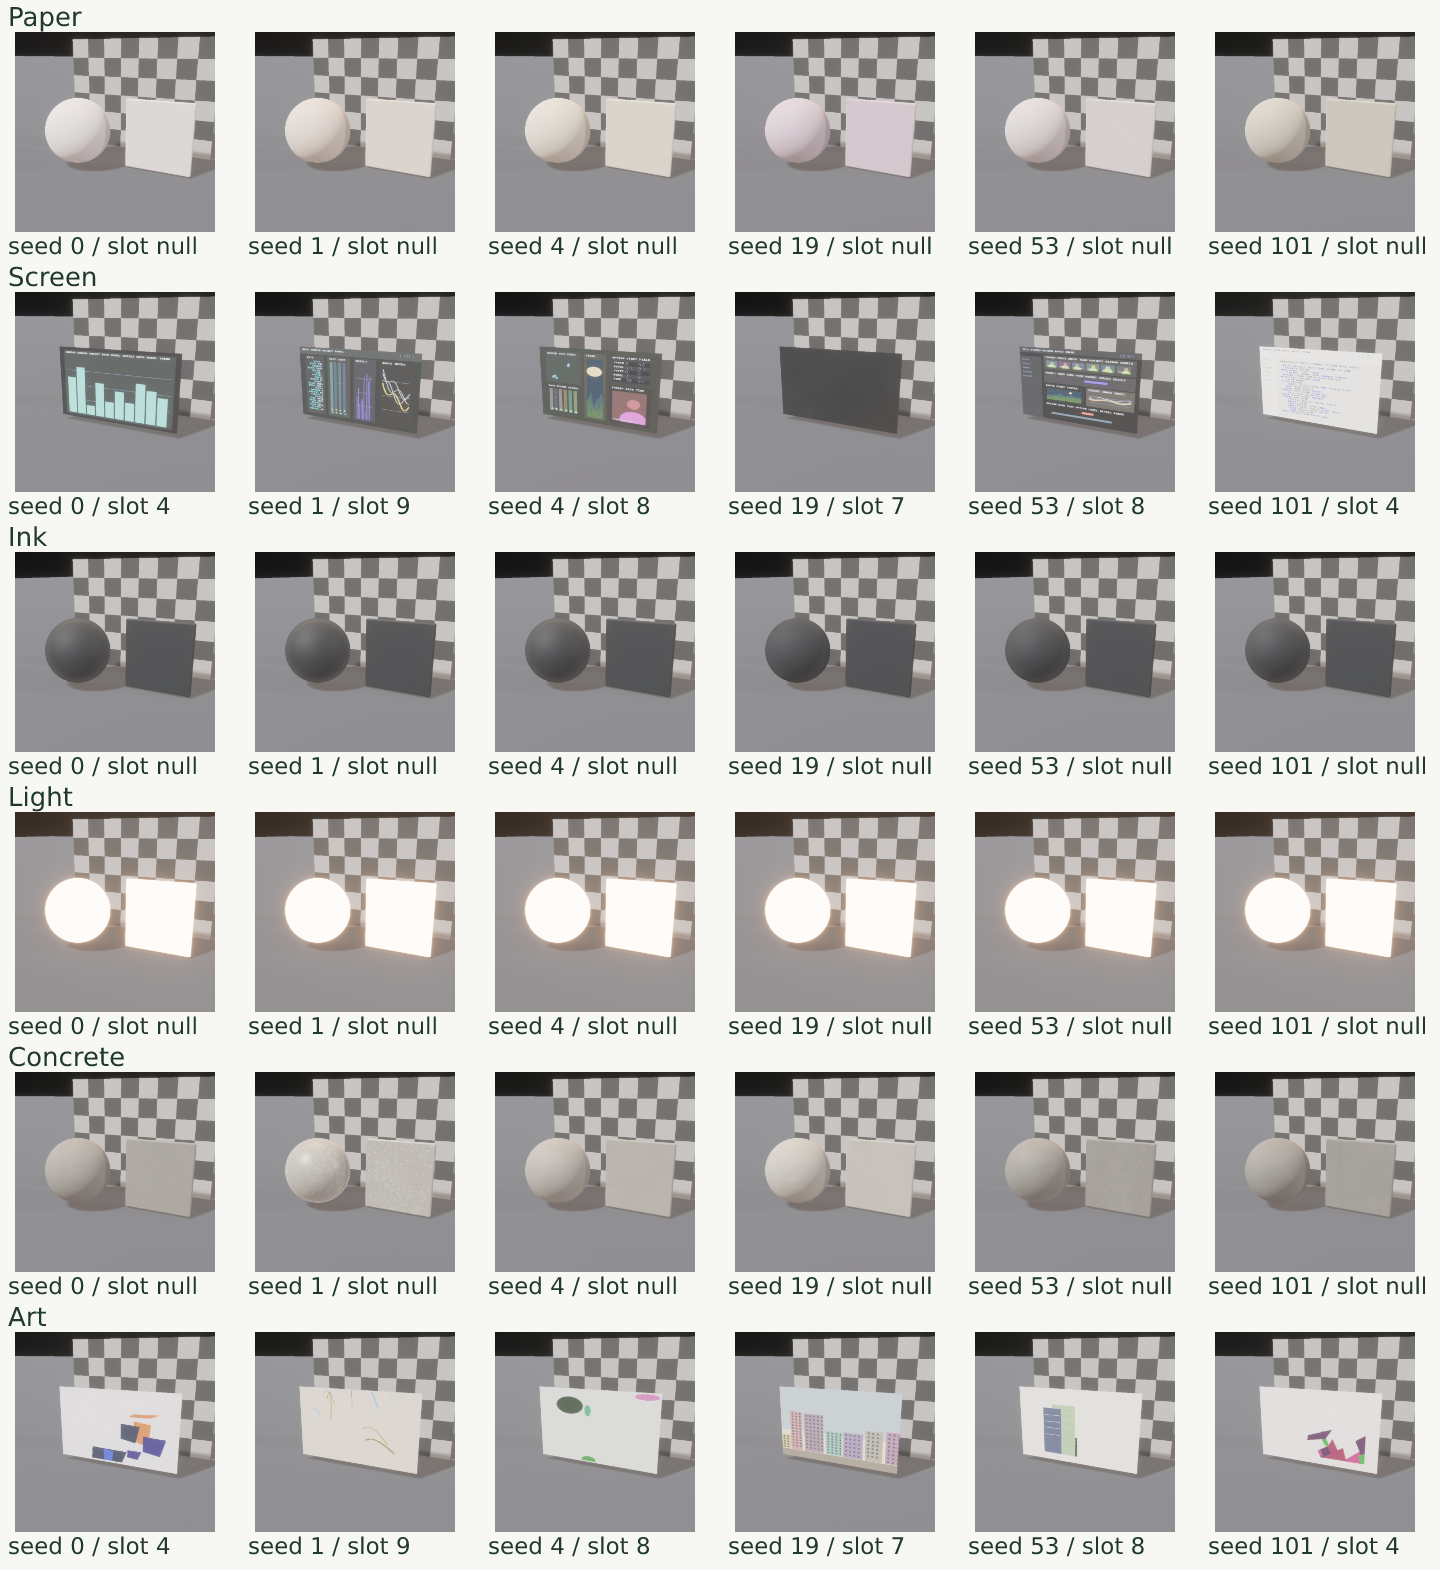
\includegraphics[width=\linewidth,height=.86\textheight,keepaspectratio]{generated/material_plate_3.png}
\caption{Native PBR material probes: Paper, Screen, Ink, Light, Concrete, Art. Columns share seed, camera, lights and geometry within each row; correlated production recipes and finish slots vary. Null slots use the base role. Six fixed examples illustrate, rather than estimate, the sampled distribution. Inspect the complete 256-seed marginals, map channels and actual PBR multipliers in the project-page atlas.}
\end{figure}
\begin{figure}[p]
\centering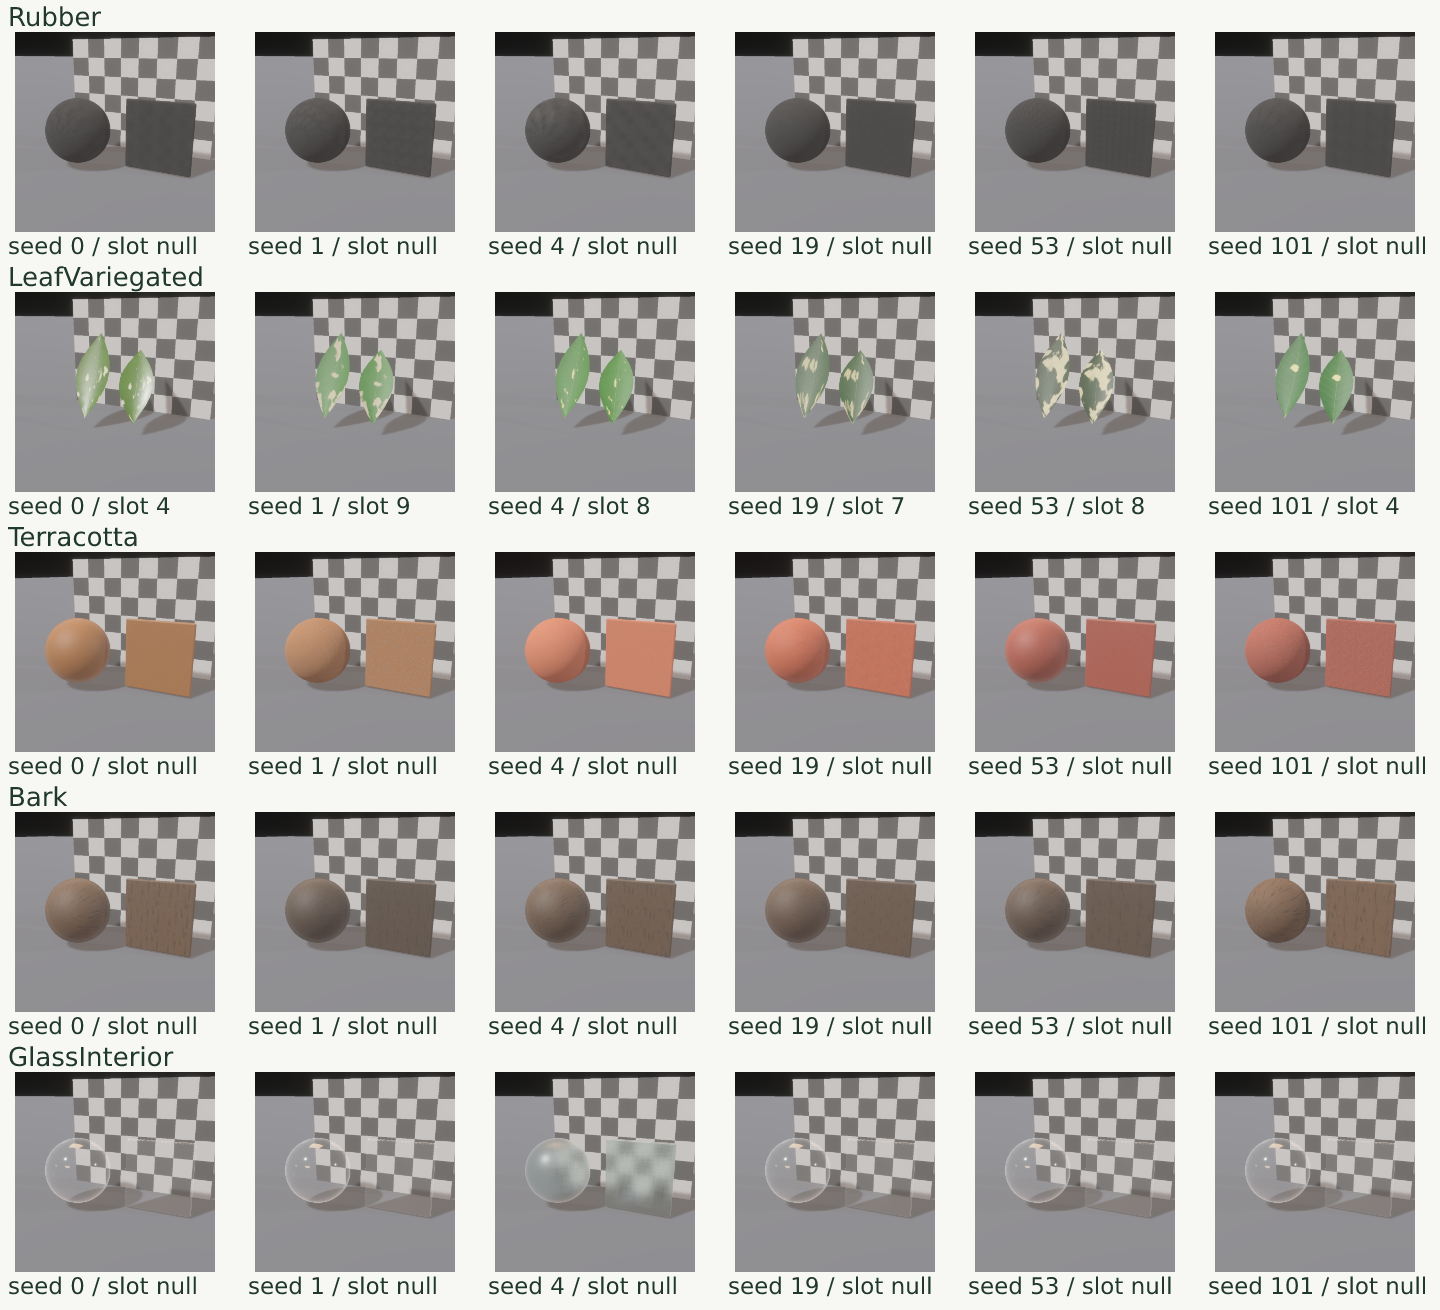
\includegraphics[width=\linewidth,height=.86\textheight,keepaspectratio]{generated/material_plate_4.png}
\caption{Native PBR material probes: Rubber, LeafVariegated, Terracotta, Bark, GlassInterior. Columns share seed, camera, lights and geometry within each row; correlated production recipes and finish slots vary. Null slots use the base role. Six fixed examples illustrate, rather than estimate, the sampled distribution. Inspect the complete 256-seed marginals, map channels and actual PBR multipliers in the project-page atlas.}
\end{figure}
\begin{figure}[p]
\centering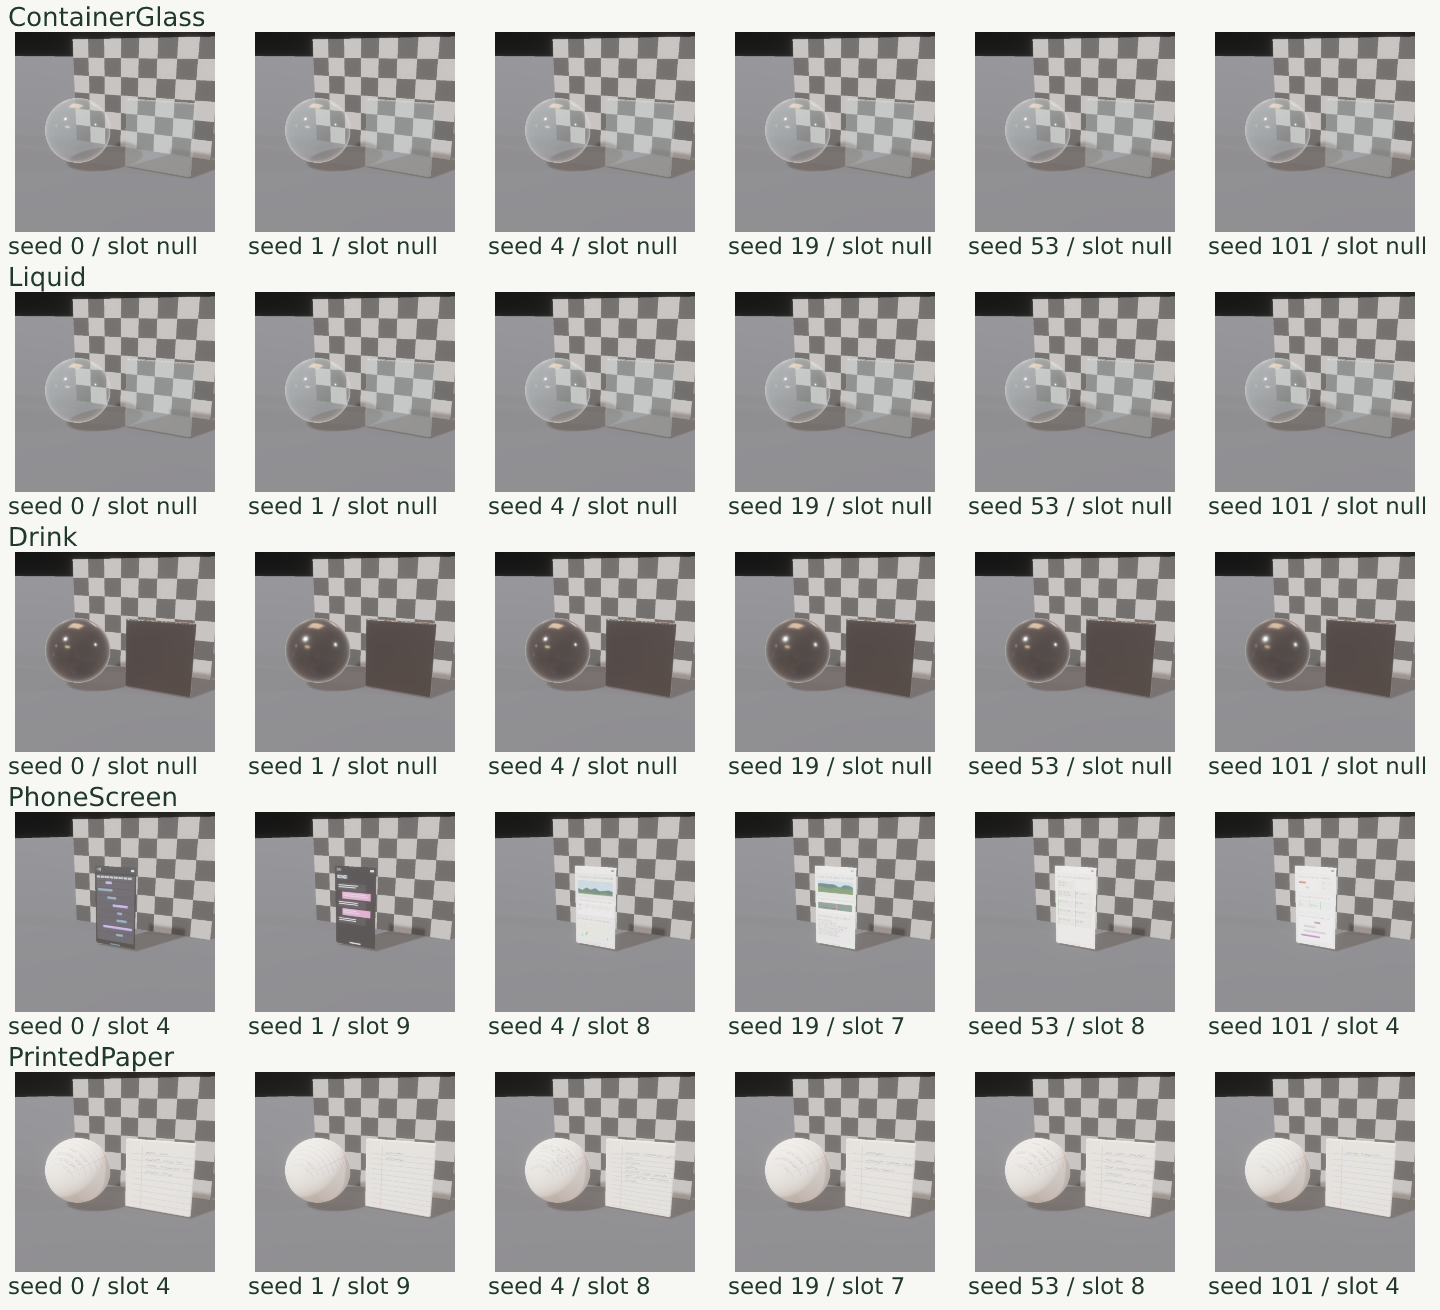
\includegraphics[width=\linewidth,height=.86\textheight,keepaspectratio]{generated/material_plate_5.png}
\caption{Native PBR material probes: ContainerGlass, Liquid, Drink, PhoneScreen, PrintedPaper. Columns share seed, camera, lights and geometry within each row; correlated production recipes and finish slots vary. Null slots use the base role. Six fixed examples illustrate, rather than estimate, the sampled distribution. Inspect the complete 256-seed marginals, map channels and actual PBR multipliers in the project-page atlas.}
\end{figure}
\begin{figure}[p]
\centering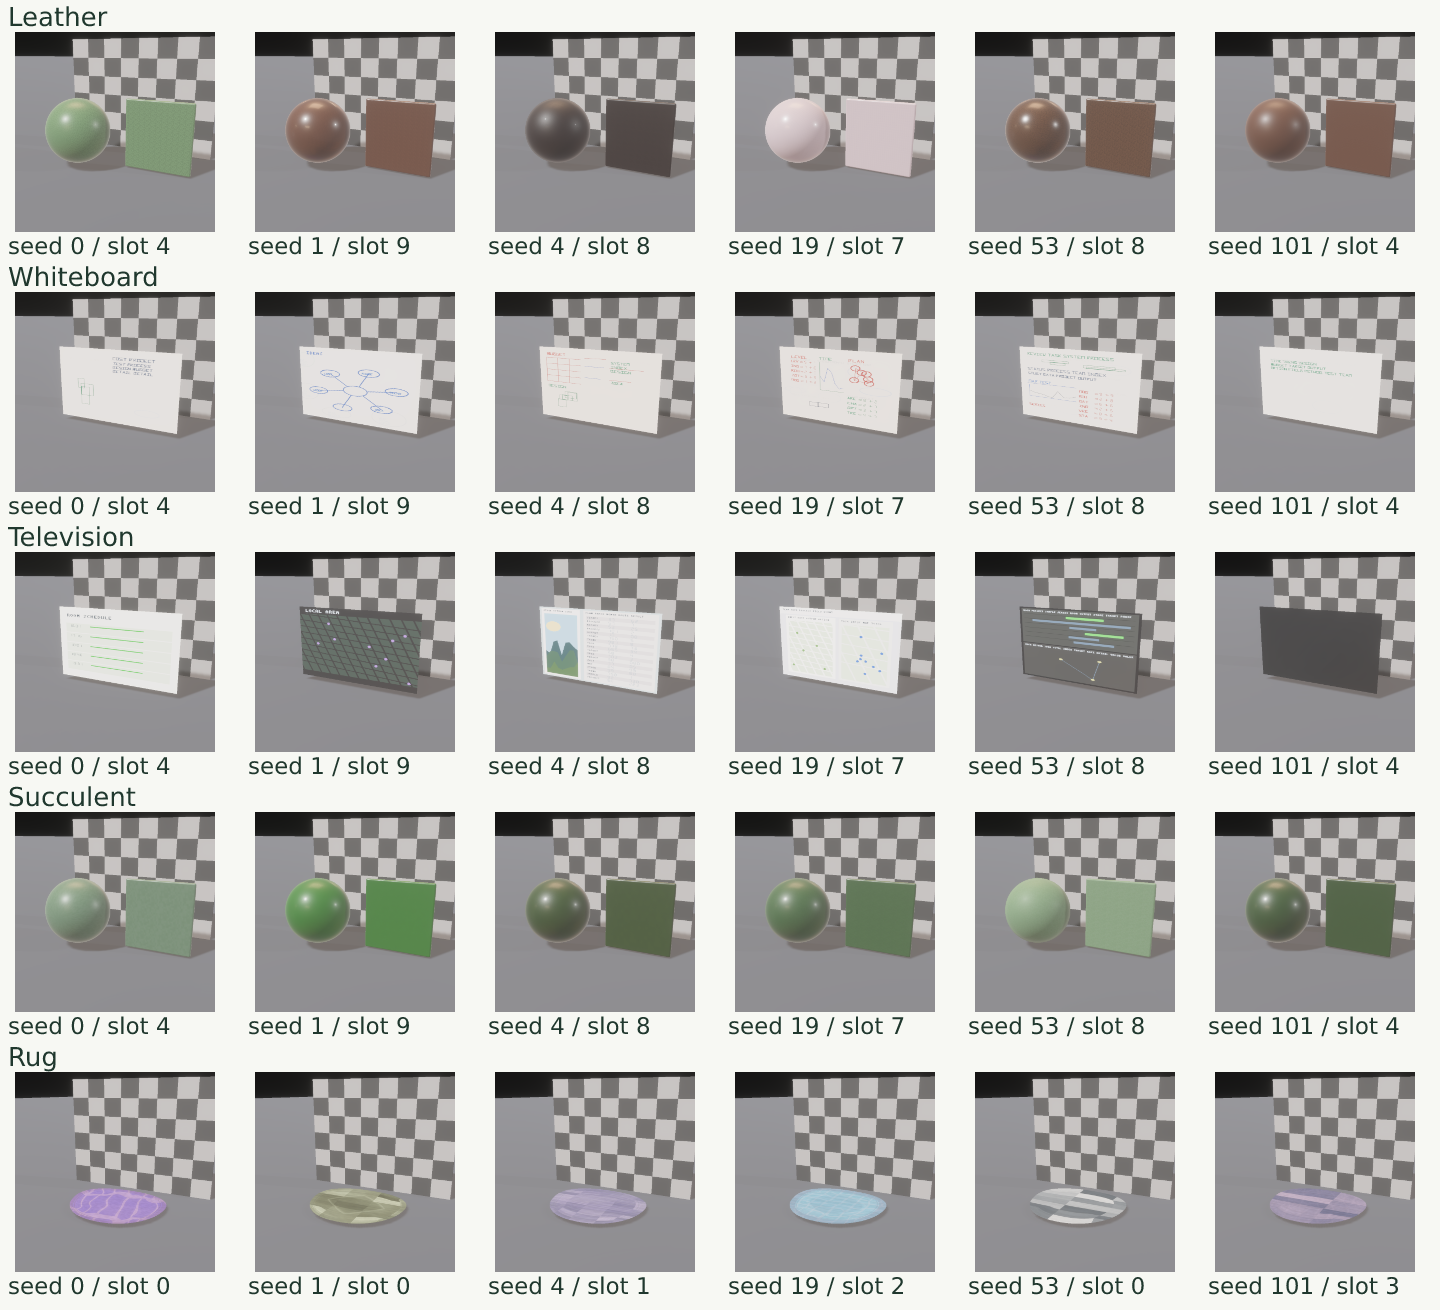
\includegraphics[width=\linewidth,height=.86\textheight,keepaspectratio]{generated/material_plate_6.png}
\caption{Native PBR material probes: Leather, Whiteboard, Television, Succulent, Rug. Columns share seed, camera, lights and geometry within each row; correlated production recipes and finish slots vary. Null slots use the base role. Six fixed examples illustrate, rather than estimate, the sampled distribution. Inspect the complete 256-seed marginals, map channels and actual PBR multipliers in the project-page atlas.}
\end{figure}
\clearpage
\subsection{A parameter-linked example: ceramic}
The following columns are the same six Ceramic images in the material plates. Recipe controls and final shader multipliers are shown separately. Glaze gloss drives the coating program; the roughness map retains local spatial detail. This is a correlated draw, not six isolated gloss interventions.
\begin{table}[h]
\centering\small
\begin{tabular}{lrrrrrr}
\toprule Material seed & 0 & 1 & 4 & 19 & 53 & 101 \\\midrule
Texture structure & 1.000 & 0.000 & 2.000 & 1.000 & 2.000 & 1.000 \\
Glaze gloss & 0.792 & 0.624 & 0.948 & 0.840 & 0.412 & 0.184 \\
Crackle strength & 0.000 & 0.000 & 0.135 & 0.230 & 0.000 & 0.000 \\
Relief (mm) & 0.059 & 0.024 & 0.052 & 0.059 & 0.020 & 0.017 \\
Shader roughness multiplier & 0.943 & 0.867 & 0.980 & 0.927 & 0.907 & 0.933 \\
Shader clearcoat & 0.206 & 0.256 & 0.419 & 0.257 & 0.179 & 0.051 \\
\bottomrule\end{tabular}
\caption{Recorded recipe values and actual PBR bindings for the Ceramic grid. Full seed records and observed ranges for every material category accompany the project page.}
\end{table}
